\documentclass[11pt]{article}
\usepackage{tikz}
\usetikzlibrary{arrows, graphs}
\usepackage{amsfonts,amssymb,amsmath,latexsym,amsthm}
\usepackage[colorlinks=true,allcolors=blue,backref=page]{hyperref}

\begin{document}

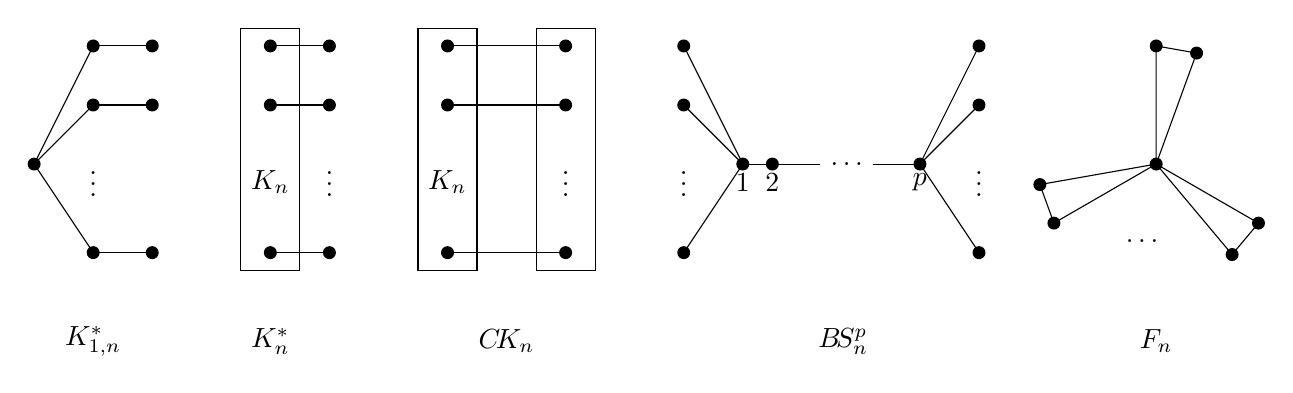
\begin{tikzpicture}[baseline=10pt,scale=0.75]
	\filldraw[fill=black,draw=black] (0,0) circle (0.1);
	\filldraw[fill=black,draw=black] (1,2) circle (0.1);
	\filldraw[fill=black,draw=black] (1,1) circle (0.1);
	\node at (1,-0.2) {$\vdots$};
	\filldraw[fill=black,draw=black] (1,-1.5) circle (0.1);
	\filldraw[fill=black,draw=black] (2,2) circle (0.1);
	\filldraw[fill=black,draw=black] (2,1) circle (0.1);
	\filldraw[fill=black,draw=black] (2,-1.5) circle (0.1);
	\draw (0,0) -- (1,2);
	\draw (0,0) -- (1,1);
	\draw (0,0) -- (1,-1.5);
	\draw (2,2) -- (1,2);
	\draw (2,1) -- (1,1);
	\draw (2,-1.5) -- (1,-1.5);
	\node at (1,-3) {$K_{1,n}^*$};

	\draw (3.5,-1.8) rectangle (4.5,2.3);
	\filldraw[fill=black,draw=black] (4,-1.5) circle (0.1);
	\filldraw[fill=black,draw=black] (4,1) circle (0.1);
	\filldraw[fill=black,draw=black] (4,2) circle (0.1);
	\node at (5,-0.2) {$\vdots$};
	\node at (4,-0.3) {$K_n$};
	\filldraw[fill=black,draw=black] (5,-1.5) circle (0.1);
	\filldraw[fill=black,draw=black] (5,1) circle (0.1);
	\filldraw[fill=black,draw=black] (5,2) circle (0.1);
	\draw (4,-1.5) -- (5,-1.5);
	\draw (4,1) -- (5,1);
	\draw (4,2) -- (5,2);
	\node at (4,-3) {$K_{n}^*$};

	\draw (7.5,-1.8) rectangle (6.5,2.3);
	\draw (8.5,-1.8) rectangle (9.5,2.3);
	\filldraw[fill=black,draw=black] (7,-1.5) circle (0.1);
	\filldraw[fill=black,draw=black] (9,-1.5) circle (0.1);
	\filldraw[fill=black,draw=black] (7,1) circle (0.1);
	\filldraw[fill=black,draw=black] (9,1) circle (0.1);
	\filldraw[fill=black,draw=black] (7,2) circle (0.1);
	\filldraw[fill=black,draw=black] (9,2) circle (0.1);
	\draw (7,-1.5) -- (9,-1.5);
	\draw (7,1) -- (9,1);
	\draw (7,2) -- (9,2);
	\node at (9,-0.2) {$\vdots$};
	\node at (7,-0.3) {$K_n$};
	\node at (8,-3) {$C\!K_n$};


	\begin{scope}[shift={(-0.5,0)}]
		\filldraw[fill=black,draw=black] (11.5,-1.5) circle (0.1);
		\filldraw[fill=black,draw=black] (11.5,1) circle (0.1);
		\filldraw[fill=black,draw=black] (11.5,2) circle (0.1);
		\filldraw[fill=black,draw=black] (12.5,0) circle (0.1);
		\node at (11.5,-0.2) {$\vdots$};

		\filldraw[fill=black,draw=black] (16.5,-1.5) circle (0.1);
		\filldraw[fill=black,draw=black] (16.5,1) circle (0.1);
		\filldraw[fill=black,draw=black] (16.5,2) circle (0.1);
		\filldraw[fill=black,draw=black] (15.5,0) circle (0.1);
		\node at (16.5,-0.2) {$\vdots$};

		\filldraw[fill=black,draw=black] (13,0)node[below]{$2$} circle (0.1);
		\draw (11.5,-1.5) -- (12.5,0);
		\draw (11.5,1) -- (12.5,0);
		\draw (11.5,2) -- (12.5,0);
		\draw(12.5,0)node[below]{$1$} -- (13.8,0);
		\draw(14.7,0) -- (15.5,0);
		\draw (16.5,-1.5) -- (15.5,0)node[below]{$p$};
		\draw (16.5,1) -- (15.5,0);
		\draw (16.5,2) -- (15.5,0);

		\node at (14.3,0) {$\dots$};
		\node at (14.2,-3) {$B\!S_n^p$};	
	\end{scope}

	\filldraw[shift ={(19,0)}][fill=black,draw=black] (0:0) circle (0.1);
	\filldraw[shift ={(19,0)}][fill=black,draw=black] (90:2) circle (0.1);
	\filldraw[shift ={(19,0)}][fill=black,draw=black] (70:2) circle (0.1);
	\filldraw[shift ={(19,0)}][fill=black,draw=black] (210:2) circle (0.1);
	\filldraw[shift ={(19,0)}][fill=black,draw=black] (190:2) circle (0.1);
	\filldraw[shift ={(19,0)}][fill=black,draw=black] (330:2) circle (0.1);
	\filldraw[shift ={(19,0)}][fill=black,draw=black] (310:2) circle (0.1);
	\node at (18.8,-1.3) {$\dots$};
	\node at (19,-3){$F_n$};
	\draw[shift ={(19,0)}] (0:0)--(90:2)--(70:2)--cycle;
	\draw [shift ={(19,0)}](0:0)--(210:2)--(190:2)--cycle;
	\draw[shift ={(19,0)}] (0:0)--(330:2)--(310:2)--cycle;
\end{tikzpicture}

\end{document}